\documentclass[11pt,a4paper]{article}
\usepackage[margin=2.4cm]{geometry}
\usepackage{amsmath,amssymb}
\usepackage{graphicx}
\usepackage{xcolor}
\usepackage{booktabs}
\usepackage[round,sort&compress]{natbib}
\usepackage[colorlinks=true,linkcolor=blue!50!black,citecolor=blue!50!black,urlcolor=blue!50!black]{hyperref}
\usepackage{caption}
\captionsetup{font=small,labelfont=bf}
\usepackage{microtype}
% Zenodo DOI of the archived bq-galaxy-models release (v1.0-sparc-cl-scaling)
\newcommand{\codeDOI}{\href{https://doi.org/10.5281/zenodo.23339753}{10.5281/zenodo.23339753}}

\newcommand{\vL}{v_{\!L}}
\newcommand{\sCL}{s_{\rm CL}}
\newcommand{\sat}{s_{\rm atan}}
\newcommand{\sdat}{s_{\rm data}}
\newcommand{\Sin}{\Sigma_{\rm in}}
\newcommand{\Mbar}{M_{\rm bar}}
\newcommand{\Vf}{V_{\rm flat}}
\newcommand{\kms}{km\,s$^{-1}$}

\title{\textbf{The central velocity gradient--surface brightness relation and the baryonic Tully--Fisher relation in two-parameter constant-Lagrangian fits to SPARC}}
\author{E.\,P.\,J. de Haas\\[2pt]
\small Kandinsky College, Nijmegen, The Netherlands \quad \href{mailto:haas2u@gmail.com}{haas2u@gmail.com}}
\date{October 2026}

\begin{document}
\maketitle

\begin{abstract}
\noindent
\citet{Lelli2013} showed that the central circular-velocity gradient of disc galaxies, $d_RV(0)$, scales with the central surface brightness as $d_RV(0)\propto I_0^{\approx0.55}$, close to the $I_0^{1/2}$ expected when the central dynamical density tracks the central stellar density. We examine how this relation, together with the baryonic Tully--Fisher relation (BTFR), appears in the two parameters $(M,R)$ of the constant-Lagrangian (CL) rotation-curve model fitted to 175 SPARC galaxies. The inner branch of the CL curve is that of a homogeneous sphere to within the small Hubble term, so the model gradient is $\sCL^2\simeq GM/R^3$ (exact for $H_z=0$) and the plateau speed is $\vL^2\simeq3GM/R$; the two relations are therefore relations between photometry and the two combinations $M/R^3$ and $M/R$. For 131 well-constrained galaxies, $\sCL$ correlates with the 3.6\,$\mu$m surface brightness at the innermost radius with Spearman $\rho=0.76$ and a bisector slope of $0.45$ ($0.41$--$0.50$), inside the range $0.38$--$0.63$ allowed by \citet{Lelli2013}, while the ordinary and inverse regression slopes ($0.35$ and $0.56$) bracket their value; using the extrapolated exponential-disc central brightness instead lowers $\rho$ to $0.58$, as their analysis anticipates for galaxies with a central light excess. $\sCL$ agrees in the median with the inner secant slope measured directly from the data (median ratio $1.01$), and $\vL$ tracks $\Vf$ to $0.03$\,dex, giving a BTFR scatter of $0.249$\,dex against $0.226$\,dex with $\Vf$. A control analysis with the arctan rotation curve of \citet{Courteau1997} yields the same correlations and slightly better fits, but a central gradient 38\% above the measured secant slope and a BTFR scatter of $0.297$\,dex. For the selected sample, combining the two relations predicts each rotation curve from baryonic quantities to within a typical factor of $1.25$ ($0.097$\,dex), equally well for both models. The CL parameters thus encode both SPARC scaling relations with a direct physical reading, while the relations themselves are not unique to the CL form. Refitting the CL model in velocity rather than squared-velocity space leaves the principal results essentially unchanged. All fits, code and data are public.
\end{abstract}

\section{Introduction}

Two empirical regularities link the visible matter of disc galaxies to their rotation. In the outer parts, the baryonic Tully--Fisher relation (BTFR) ties the total baryonic mass to the flat rotation speed with very small intrinsic scatter \citep{McGaugh2000,Lelli2016btfr,Lelli2019}. In the inner parts, \citet{Lelli2013} found that the circular-velocity gradient for $R\to0$, $d_RV(0)$, correlates with the observed central surface brightness $\mu_0$ over two orders of magnitude in gradient and four in surface brightness,
\begin{equation}
\log d_RV(0) = (-0.22\pm0.02)\,\mu_0 + (6.28\pm0.40),
\label{eq:lelli}
\end{equation}
for their full sample of 52 galaxies, which includes S0/Sa galaxies with less certain gradients, with $\mu_0$ in R-band magnitudes. In linear surface brightness, $d_RV(0)\propto I_0^{0.55}$. The authors estimate that systematics confine the true slope to between $-0.15$ and $-0.25$ mag$^{-1}$, i.e.\ $I_0^{0.38}$ to $I_0^{0.63}$, and note that a slope of exactly $0.5$ follows when the central dynamical density is a fixed multiple of the central baryonic density, which would require a puzzling fine-tuning between the 3D distribution of the baryons, the thickness and mass-to-light ratio of the central component, and its baryon fraction.

The constant-Lagrangian (CL) model \citep{deHaas2018,deHaas2025a,deHaas2025b} describes a rotation curve with two parameters, a mass $M$ and a radius $R$, plus the Hubble rate $H_z$ held fixed. It was fitted to all 175 galaxies of the SPARC database \citep{Lelli2016sparc}, and the fits, with per-galaxy atlases and interactive models, are public at \url{https://haas2u-ai.github.io/bq-galaxy-models/}. Because the inner branch of the CL curve is solid-body and the outer branch tends to a plateau, the two parameters map naturally onto an inner gradient and an outer speed. This paper asks three questions: (i) do the fitted parameters reproduce the gradient--surface brightness relation of \citet{Lelli2013} and the BTFR, (ii) what part of that agreement is specific to the CL form rather than a property of any reasonable two-parameter curve, and (iii) what the CL parameters add to the physical reading of the relations. To answer (ii), every step is repeated with the arctan rotation curve of \citet{Courteau1997}.

The CL rotation law was introduced as an empirical postulate \citep{deHaas2018} and has since been derived within a relativistic Spin(1,3) rotor formulation of gravitational vacuum flow. The construction is developed in a biquaternion algebra, lifted to the Weyl representation of the Clifford algebra Cl(1,3), and shown to carry over unchanged to Spacetime Algebra and to the Dirac-matrix formalism \citep{deHaasSpin}. It is rapidity-first rather than metric-first: the Lorentz rotor is the primary object, and the spacetime metric follows from it as a derived projection, which in the slow-flow limit is the Painlev\'e--Gullstrand (PG) metric \citep{Painleve1921,Gullstrand1922} in its river-model reading \citep{Hamilton2008,deHaasMC}. Newtonian gravity itself is left unchanged.

In the river model, space flows radially inward at the Newtonian escape speed $v_N=\sqrt{2GM/r}$; here that river is combined with the Hubble flow $v_H=H_zr$ into the effective radial flow $v_{r,\rm eff}=v_N-v_H$, the Newton--Hubble PG riverbed, which has also appeared in vacuum-flow descriptions of galactic dynamics \citep{Wong2016}, which defines the radial rapidity $\chi_r=v_{r,\rm eff}/c$. The step that leads to the CL law is the addition of a second, azimuthal component to this purely radial river. The gravitational rapidity field becomes $\chi_g=(\chi_r,\chi_\phi)$, in which $\chi_r$ is fixed by the source while the azimuthal rapidity $\chi_\phi$ is not prescribed but is a dynamical degree of freedom: the self-organised response of the flow to the radial inflow \citep{deHaasSpin}. The two compose through the ordered Spin(1,3) rotor $G=G_\phi G_r$ \citep{deHaasGFD,deHaasRapidity}, whose non-commuting boosts also generate a Thomas--Wigner rotation channel. Two independent routes lead from this rotor to the same transport law. In the kinematic route the time component of the convective four-acceleration is $a_0=c\,D\Gamma/D\tau$; in the connection route the proper-time Maurer--Cartan connection $\Omega_\tau=(D_\tau G)\,G^{-1}$, transported with the gravitational four-velocity $U_g$, has time channel $[U_g\Omega_\tau]_{\hat T}=\tfrac{c}{2}\,D\Gamma/D\tau$ \citep{deHaasMC,deHaasSpin}. Both vanish when the composed Lorentz factor $\Gamma=\cosh\chi_r\cosh\chi_\phi$ is conserved along each flow line, $D\Gamma/D\tau=0$. Radial and azimuthal rapidity are then exchanged while the total hyperbolic boost stays fixed, so that every streamline lies on a curve of constant composed rapidity \citep{deHaasRapidity}. In the slow-flow limit, $c^2(\Gamma-1)\to\tfrac12(v_{r,\rm eff}^2+v_\phi^2)$, and this isorapidity condition reduces to the constant-Lagrangian relation $v_\phi^2+v_{r,\rm eff}^2=\vL^2$ on $R\le r\le r_c$, where $r_c=(2GM/H_z^2)^{1/3}$ is the radius at which the radial flow stalls. A Newtonian virial closure at the core--exterior transition at $R$, $v_\phi^2(R)=\tfrac12v_{r,\rm eff}^2(R)$, fixes $\vL^2=\tfrac32v_{r,\rm eff}^2(R)$; inside $R$ the model takes the solid-body form. Together these give the rotation curve of Eq.~(\ref{eq:cl}).

In this construction $M$ is the mass that drives the radial inflow and $R$ the radius at which the virial closure holds; both are theoretical quantities rather than photometric ones, and the present paper does not depend on that interpretation. At fixed $H_z$ the map
\begin{equation}
(M,R)\;\longmapsto\;(\vL,\sCL),\qquad \vL=\sqrt{\tfrac32}\left(\sqrt{\frac{2GM}{R}}-H_zR\right),\qquad \sCL=\frac{\vL}{\sqrt3\,R},
\label{eq:map}
\end{equation}
is one-to-one, so every fitted curve is described equally well by its plateau speed $\vL$ and its central gradient $\sCL$, the model quantities that are compared with the observed $\Vf$ and $d_RV(0)$. Replacing $(M,R)$ by $(\vL,\sCL)$ is the step from theory to phenomenology taken in this paper: the tests below concern only the fitted curves and the observed light, and their outcome does not depend on how $M$ and $R$ are interpreted.

\section{Data, models and fits}
\label{sec:data}

\subsection{SPARC}
We use the SPARC rotation curves and 3.6\,$\mu$m photometry of \citet{Lelli2016sparc}: 175 galaxies with $V_{\rm obs}(r)$, its random error, and the disc and bulge surface-brightness profiles tabulated at the rotation-curve radii. Baryonic masses are $\Mbar=\Upsilon_d L_{\rm disc}+\Upsilon_b L_{\rm bul}+1.33\,M_{\rm HI}$ with the SPARC values $\Upsilon_d=0.5$ and $\Upsilon_b=0.7$\,M$_\odot$/L$_\odot$. The main sample keeps galaxies with quality flag $Q\le2$ and inclination $i\ge30^\circ$ whose CL fit constrains both parameters (Sect.~\ref{sec:fits}); it contains 131 galaxies, 14 of which have a photometric bulge.

\subsection{The CL rotation curve}
The single-Lagrangian CL curve is \citep{deHaas2018,deHaas2025b}
\begin{equation}
v^2(r)=\begin{cases}
\tfrac12 X^2\,r^2/R^2, & r\le R,\\[3pt]
\tfrac32 X^2-\left(\sqrt{2GM/r}-H_zr\right)^2, & r>R,
\end{cases}
\qquad X=\sqrt{2GM/R}-H_zR,
\label{eq:cl}
\end{equation}
with $H_z=2.2\times10^{-18}$\,s$^{-1}$ fixed. The curve rises linearly to $R$, where $v^2(R)=\tfrac12X^2$, and then approaches the plateau $\vL^2=\tfrac32X^2$. Because $w=\sqrt{2GM/r}-H_zr$ decreases monotonically to zero at $r_c=(2GM/H_z^2)^{1/3}$, $v^2$ rises monotonically towards $\vL^2$, reaches it at $r_c$, and declines only beyond $r_c$, which for most galaxies lies outside the observed radii. Hence $v^2(R)=\vL^2/3$: $R$ is the radius at which the squared rotation speed reaches one third of its plateau value.

\subsection{The arctan control}
As a control we fit the empirical curve of \citet{Courteau1997},
\begin{equation}
V(r)=\frac{2}{\pi}V_c\arctan\!\left(\frac{r}{r_t}\right),
\label{eq:atan}
\end{equation}
which also has two parameters, an asymptotic speed $V_c$ and a turnover radius $r_t$, and a central gradient $\sat=2V_c/(\pi r_t)$.

\subsection{Fitting}
\label{sec:fits}
The CL model is fitted to $V_{\rm obs}^2$ with uncertainties $2V_{\rm obs}\,\delta V_{\rm obs}$, as in \citet{deHaas2018}; the arctan curve is fitted to $V_{\rm obs}$ with $\delta V_{\rm obs}$. Both use bounded least squares in $\log$ parameters from a grid of starting points, and $1\sigma$ errors from the covariance matrix scaled by $\sqrt{\chi^2_\nu}$ when $\chi^2_\nu>1$. For 25 of the 175 galaxies, mostly massive systems with a bulge or a Keplerian outer decline, the CL radius is not constrained: in 20 it runs to its lower bound and only $M/R$ is measured, in 5 more $\sigma(\log M)>0.5$\,dex. These are excluded from the main sample. Evaluated for both models in $V$ (which is the space the arctan fit minimises), the median $\chi^2_\nu$ of the main sample is $0.96$ for CL and $0.68$ for arctan; arctan gives the lower $\chi^2_\nu$ in 62\% of the galaxies. To check that the choice of fitting space does not drive the results, we also refitted the CL model directly in $V$ with $\delta V$. All 131 main-sample galaxies remain constrained; $\log R$ changes by $-0.007$\,dex in the median (scatter $0.03$\,dex) and $\sCL$ by a factor $1.015$. The gradient relation with $\Sin$ is unchanged ($\rho=0.77$, bisector slope $0.46$ with interval $0.41$--$0.50$, median $\sCL/\sdat=1.016$), as is the BTFR (scatter $0.250$\,dex, $\vL/\Vf=1.064$); the median $\chi^2_\nu$ becomes $0.95$. We therefore quote the squared-velocity fits throughout.

\subsection{Derived quantities}
For each galaxy we compute three inner gradients: $\sCL=\vL/(\sqrt3R)$ (Sect.~\ref{sec:core}), $\sat$, and a model-independent $\sdat$, the least-squares slope through the origin of the first three rotation-curve points. As central surface brightness we use three 3.6\,$\mu$m proxies: $\Sin$, the total (disc + bulge) surface brightness at the innermost tabulated radius; $\Sigma_{\rm ex}$, a log-linear extrapolation of the first two profile points to $r=0$, not allowed to fall below $\Sin$; and $\Sigma_{d,0}$, the central surface brightness of the exponential disc fit listed by SPARC. \citet{Lelli2013} obtain their observed $\mu_0$ by extrapolating the inner few arcseconds of the profile to $r=0$, so that it keeps any central light excess; $\Sigma_{\rm ex}$ follows that procedure and $\Sin$ shares its intent, while $\Sigma_{d,0}$ corresponds to their extrapolated disc value $\mu_d$.

\section{The CL inner branch as a uniform core}
\label{sec:core}

For $r\le R$, Eq.~(\ref{eq:cl}) gives $v=(X/\sqrt2R)\,r$, so the central gradient is
\begin{equation}
\sCL=\frac{X}{\sqrt2\,R}=\frac{\vL}{\sqrt3\,R},\qquad
\sCL^2=\frac{GM}{R^3}\left(1-\frac{H_zR}{\sqrt{2GM/R}}\right)^2\simeq\frac{GM}{R^3}.
\label{eq:grad}
\end{equation}
For $H_z=0$ this is exactly the circular speed inside a homogeneous sphere of mass $M$ and radius $R$; for $H_z\neq0$ the factor in brackets defines a slightly smaller effective mass, and in the fits $\sCL^2/(GM/R^3)$ has median $0.997$. Likewise $M=\vL^2R/(3G)$ to $0.3$\% in the median. Two consequences follow.

First, Eq.~(6) of \citet{Lelli2013}, $d_RV(0)=\sqrt{\beta G\rho_{\rm dyn,0}}$ with $\beta=4\pi\alpha/3$, applies with $\alpha=1$, the spherical case, and identifies the CL central dynamical density as
\begin{equation}
\rho_{{\rm dyn},0}=\frac{3\sCL^2}{4\pi G}\simeq\frac{3M}{4\pi R^3},
\label{eq:rho}
\end{equation}
the mean density of the CL core. The gradient--surface brightness relation is therefore a relation between $M/R^3$ and photometry, while the BTFR is one between $M/R\simeq\vL^2/3G$ and photometry. The two relations constrain different combinations of the same two parameters.

Second, $R$ can be read from a rotation curve without the model, as the radius $r_{1/3}$ where $V_{\rm obs}$ first reaches $\Vf/\sqrt3$. For the 80 main-sample galaxies with a SPARC $\Vf$ and a resolved crossing, $r_{1/3}$ and the fitted $R$ correlate with $\rho=0.94$ at a median ratio of $0.90$ (Fig.~\ref{fig:R}, left). $R$ is thus an observable feature of the curve, not only a fit parameter. Figure~\ref{fig:examples} shows four examples spanning the surface-brightness range.

\begin{figure}[t]
\centering
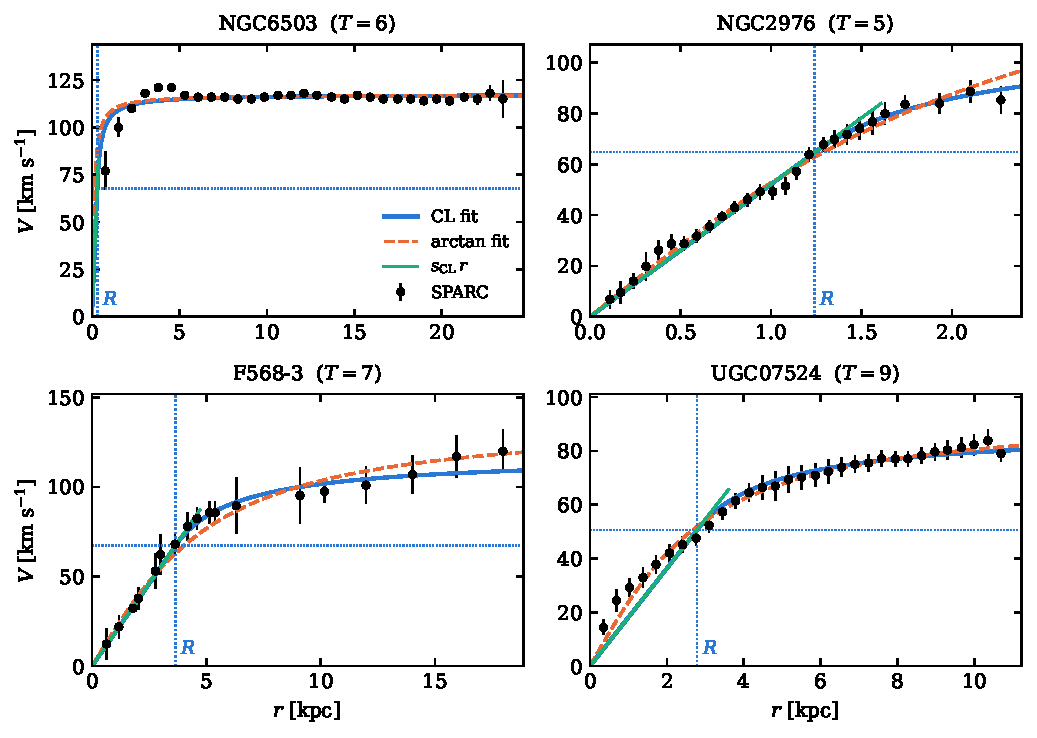
\includegraphics[width=0.86\textwidth]{fig/fig1_examples.pdf}
\caption{Example SPARC rotation curves with the CL fit (solid), the arctan fit (dashed) and the CL inner gradient $\sCL\,r$ (green). Dotted lines mark $R$ and $\vL/\sqrt3$, the speed at $R$.}
\label{fig:examples}
\end{figure}

\section{The gradient--surface brightness relation}
\label{sec:lelli}

Table~\ref{tab:lelli} lists, for each gradient estimator and surface-brightness proxy, the Spearman coefficient, the ordinary least-squares slope of $\log s$ on $\log\Sigma$, the inverse slope, the bisector slope \citep{Isobe1990} with a bootstrap 95\% interval, and the scatter about the bisector. Because both axes carry substantial scatter, the ordinary and inverse regressions give lower and higher slopes, respectively; we use the bisector as a descriptive symmetric estimate, without implying that it recovers the true structural slope. Slopes are given per dex of $\Sigma$, so the reference values are $0.55$ \citep[their Eq.~4]{Lelli2013}, the range $0.38$--$0.63$ they consider allowed, and $0.5$ for a constant central density ratio. \citet{Lelli2013} use an error-weighted linear fit of $\log d_RV(0)$ on $\mu_0$; with comparable scatter on both axes the result depends on the regression direction, so we quote all three slopes.

\begin{table}[h]
\centering
\caption{Gradient--surface brightness relation for the 131 main-sample galaxies (3.6\,$\mu$m, $\Sigma$ in L$_\odot$\,pc$^{-2}$, $s$ in \kms\,kpc$^{-1}$).}
\label{tab:lelli}
\small
\begin{tabular}{llccccc}
\toprule
Gradient & $\Sigma$ proxy & $\rho$ & OLS & inverse & bisector (95\%) & scatter [dex]\\
\midrule
$\sdat$ & $\Sin$          & 0.78 & 0.34 & 0.51 & 0.42 (0.37--0.46) & 0.22\\
        & $\Sigma_{\rm ex}$ & 0.74 & 0.31 & 0.51 & 0.41 (0.36--0.46) & 0.23\\
        & $\Sigma_{d,0}$ & 0.55 & 0.25 & 1.08 & 0.59 (0.50--0.69) & 0.38\\
\midrule
$\sCL$  & $\Sin$          & 0.76 & 0.35 & 0.56 & 0.45 (0.41--0.50) & 0.25\\
        & $\Sigma_{\rm ex}$ & 0.77 & 0.34 & 0.54 & 0.44 (0.39--0.48) & 0.24\\
        & $\Sigma_{d,0}$ & 0.58 & 0.28 & 1.12 & 0.62 (0.52--0.73) & 0.40\\
\midrule
$\sat$  & $\Sin$          & 0.78 & 0.41 & 0.64 & 0.52 (0.47--0.57) & 0.28\\
        & $\Sigma_{\rm ex}$ & 0.79 & 0.41 & 0.62 & 0.51 (0.45--0.56) & 0.27\\
        & $\Sigma_{d,0}$ & 0.59 & 0.33 & 1.27 & 0.70 (0.59--0.81) & 0.45\\
\bottomrule
\end{tabular}
\end{table}

The relation is clearly present in the CL parameters. With $\Sin$, $\sCL$ correlates at $\rho=0.76$ with a bisector slope of $0.45$, broadly consistent with \citet{Lelli2013}: inside their allowed range and close to $0.5$ (Fig.~\ref{fig:lelli}); the ordinary slope ($0.35$) falls below that range and the inverse slope ($0.56$) matches their value, so a like-for-like comparison of normalisation-free slopes is only possible within these bounds. The choice of surface-brightness proxy matters in the way \citet{Lelli2013} describe: replacing the observed central light by the extrapolated disc value $\Sigma_{d,0}$ reduces $\rho$ from $0.76$ to $0.58$ and nearly doubles the scatter. In the 14 bulge galaxies $\Sin$ exceeds $\Sigma_{d,0}$ by a median $0.57$\,dex; these galaxies sit at the high end of the relation, and their rms deviation about the fitted relation grows from $0.30$\,dex with $\Sin$ to $0.73$\,dex with $\Sigma_{d,0}$. The correlation is not merely inherited from galaxy size: holding $\Vf$ fixed, the partial Spearman coefficient between $\sCL$ and $\Sin$ remains $0.61$ (101 galaxies).

\begin{figure}[t]
\centering
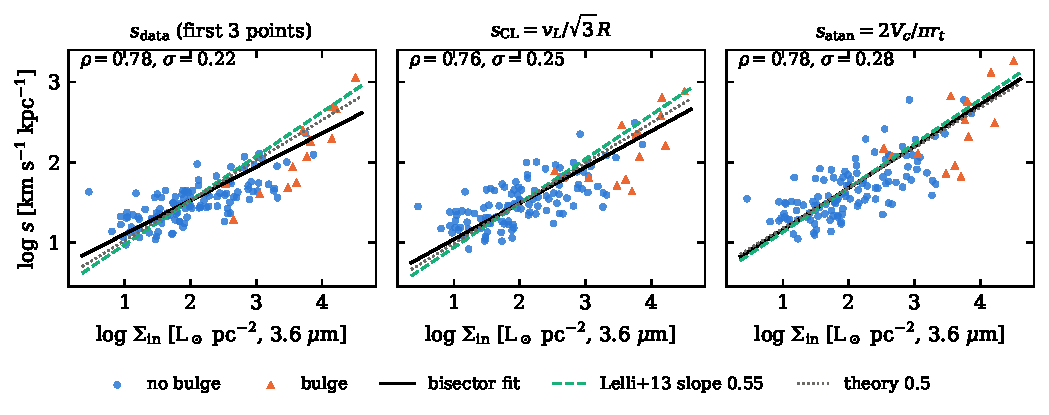
\includegraphics[width=\textwidth]{fig/fig2_gradient_SB.pdf}
\caption{Central velocity gradient against 3.6\,$\mu$m surface brightness at the innermost radius for the gradient measured from the data (left), the CL gradient (middle) and the arctan gradient (right). Black: bisector fit. Green dashed: the slope $0.55$ of \citet{Lelli2013}; grey dotted: slope $0.5$; both drawn through the sample medians, since the normalisation differs between R band and 3.6\,$\mu$m. Triangles: galaxies with a photometric bulge.}
\label{fig:lelli}
\end{figure}

\paragraph{What is specific to CL.} The control shows that the correlation itself is not. With $\Sin$, $\sdat$, $\sCL$ and $\sat$ give the same $\rho$ within $0.02$ (within $0.05$ for the other proxies), and $\sCL$ and $\sat$ are almost perfectly rank-correlated ($\rho=0.99$); their residuals about the respective relations correlate at $0.97$. What differs is the normalisation (Fig.~\ref{fig:agree}). The CL gradient agrees in the median with the measured inner secant slope, $\sCL/\sdat=1.01$ ($\rho=0.85$), whereas the arctan gradient exceeds it by a median factor $1.38$, because the arctan curve bends continuously and its slope at the origin is steeper than the secant through the inner points. This difference is not necessarily a bias of the arctan form: for a curve that is concave near the centre, a secant through finite radii underestimates the true derivative at the origin, so $\sat$ may be closer to $d_RV(0)$ where the inner rise is resolved. The CL form, whose inner branch is strictly linear up to $R$, has a central derivative equal to its secant and so represents the inner rise in the form in which it is measured. This also explains why the bisector slope for $\sat$ is somewhat steeper than for $\sdat$ and $\sCL$.

\begin{figure}[t]
\centering
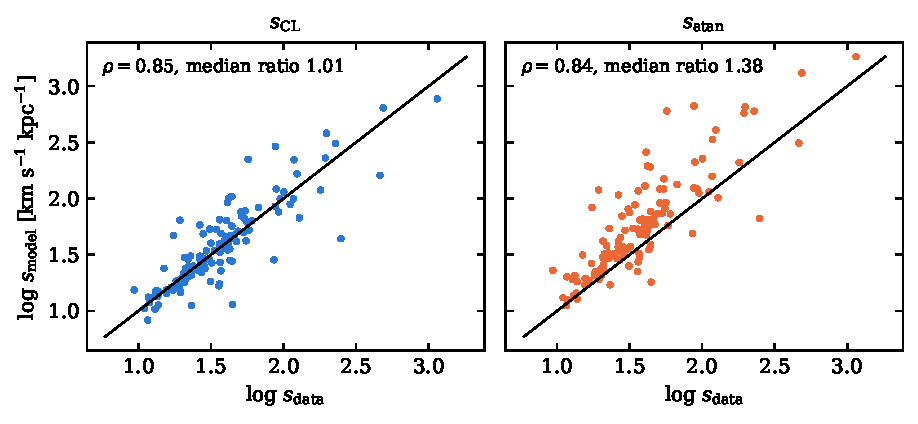
\includegraphics[width=0.78\textwidth]{fig/fig3_gradient_agreement.pdf}
\caption{Model gradients against the gradient measured from the first three rotation-curve points. Line: equality.}
\label{fig:agree}
\end{figure}

\section{The baryonic Tully--Fisher relation}
\label{sec:btfr}

For the 101 main-sample galaxies with a SPARC $\Vf$, Table~\ref{tab:btfr} compares the BTFR obtained with $\Vf$, with the CL plateau $\vL$ and with the arctan asymptote $V_c$ (Fig.~\ref{fig:btfr}). $\Mbar$ does not enter either fit, so the tight relation with $\vL$ is an external check of the fitted velocity scale. It does not, however, improve on $\Vf$: $\vL=1.065\,\Vf$ with only $0.029$\,dex galaxy-to-galaxy scatter, the BTFR scatter is $0.249$\,dex against $0.226$\,dex, and the offsets from the $\Vf$ relation are uncorrelated with $\vL/\Vf$ ($\rho=-0.02$). For comparison, \citet{Lelli2019} report an observed scatter of $0.24$\,dex with $\Vf$ for 123 SPARC galaxies. The CL plateau is a closer proxy for $\Vf$ than the arctan asymptote, which scatters by $0.052$\,dex around $1.125\,\Vf$ and yields a BTFR scatter of $0.297$\,dex.

\begin{table}[h]
\centering
\caption{BTFR for 101 main-sample galaxies with SPARC $\Vf$ (ordinary least squares of $\log\Mbar$ on $\log V$).}
\label{tab:btfr}
\small
\begin{tabular}{lccc}
\toprule
Velocity & slope & scatter [dex] & $V/\Vf$ (median; scatter)\\
\midrule
$\Vf$ (SPARC) & 3.45 & 0.226 & ---\\
$\vL$ (CL) & 3.54 & 0.249 & 1.065; 0.029 dex\\
$V_c$ (arctan) & 3.66 & 0.297 & 1.125; 0.052 dex\\
\bottomrule
\end{tabular}
\end{table}

\begin{figure}[t]
\centering
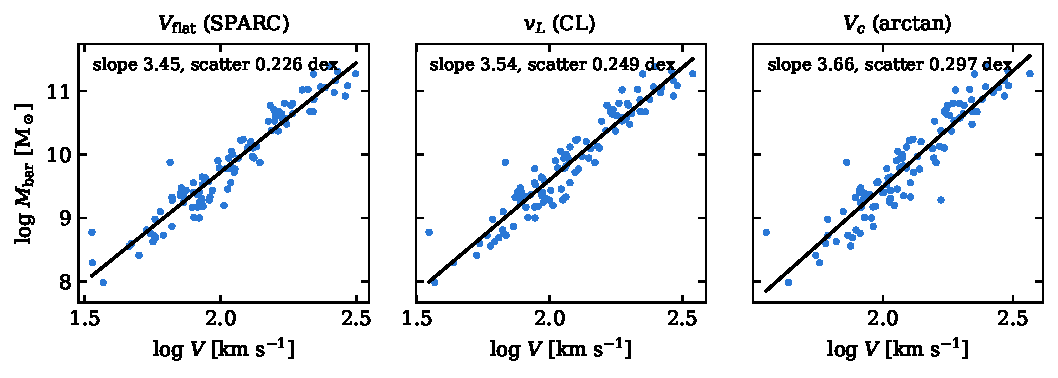
\includegraphics[width=\textwidth]{fig/fig4_btfr.pdf}
\caption{BTFR with the observed flat speed, the CL plateau speed and the arctan asymptotic speed.}
\label{fig:btfr}
\end{figure}

\section{R as a structural scale}
\label{sec:R}

The fitted $R$ follows the photometric disc scale length $R_d$ ($\rho=0.40$), with median $R/R_d=0.90$, inside the radius $2.2R_d$ where a pure exponential disc's rotation curve peaks. The ratio $R/R_d$ rises steadily along the Hubble sequence ($\rho=0.65$ with type $T$; Fig.~\ref{fig:R}, right) and falls with surface brightness ($\rho=-0.61$ with $\Sin$): in early-type and high-surface-brightness discs the CL core is compact relative to the light, in late-type and low-surface-brightness discs it extends beyond $R_d$. This is the CL expression of the familiar contrast between steeply and slowly rising rotation curves. The arctan turnover radius shows the same trend ($\rho=0.69$ for $r_t/R_d$ with $T$), so the trend is a property of the data; the CL contribution is to attach it to a scale with a definite kinematic meaning, the one-third point of $v^2$.

\begin{figure}[t]
\centering
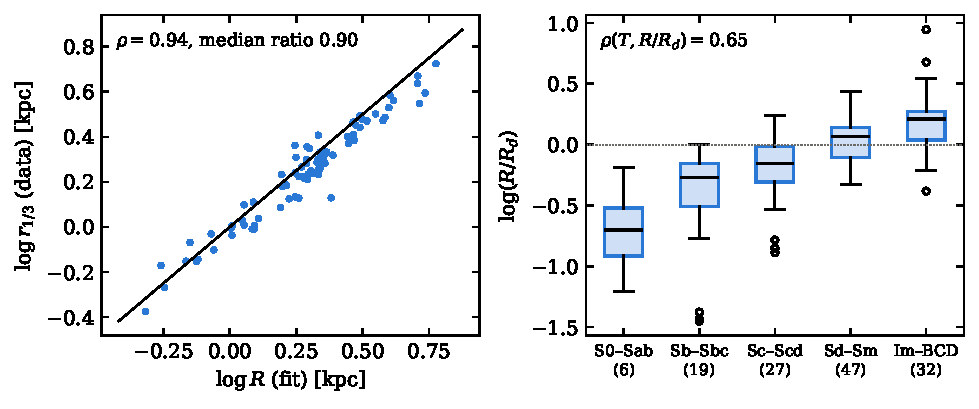
\includegraphics[width=0.84\textwidth]{fig/fig5_R_structure.pdf}
\caption{Left: radius $r_{1/3}$ where the observed curve reaches $\Vf/\sqrt3$ against the fitted CL radius. Right: $R/R_d$ by Hubble type (number of galaxies in brackets).}
\label{fig:R}
\end{figure}

\section{Rotation curves from photometry}
\label{sec:pred}

Because a CL curve is fixed by $(\vL,R)$, the two relations together predict a rotation curve from baryonic quantities (3.6\,$\mu$m photometry and HI mass), once calibrated on the other galaxies: $\vL$ from $\Mbar$ through the BTFR, $\sCL$ from $\Sin$ through the gradient relation, $R=\vL/(\sqrt3\,\sCL)$, and $M$ from Eq.~(\ref{eq:cl}). We calibrate both relations with bisector fits in a leave-one-out scheme, so that no galaxy contributes to its own prediction, and do the same for the arctan curve with $V_c$ and $\sat$. The predicted curves match the observed ones with a median per-galaxy rms of $0.097$\,dex (a typical factor of $1.25$) for CL and $0.091$\,dex (a factor of $1.23$) for arctan, against $0.037$ and $0.027$\,dex for the fits themselves; CL is the better of the two for 49\% of the galaxies (Fig.~\ref{fig:pred}). The photometric $R$ reproduces the fitted one with $0.24$\,dex scatter. The two relations thus recover the overall amplitude and shape of most curves from $\Mbar$ (stellar light and HI) and the central light, but at roughly three times the residual of a direct fit, and the CL form does not predict better than the empirical control. Two caveats limit this test. The sample was selected partly on the CL fits being constrained, and $\Sin$ is sampled at the innermost kinematic radius, so the prediction is not independent of the rotation-curve data in the way a purely photometric one would be. By comparison, the radial acceleration relation predicts rotation curves from the baryon distribution with a single universal function, with observed scatter ``small and largely dominated by observational uncertainties'' \citep{McGaugh2016}.

\begin{figure}[t]
\centering
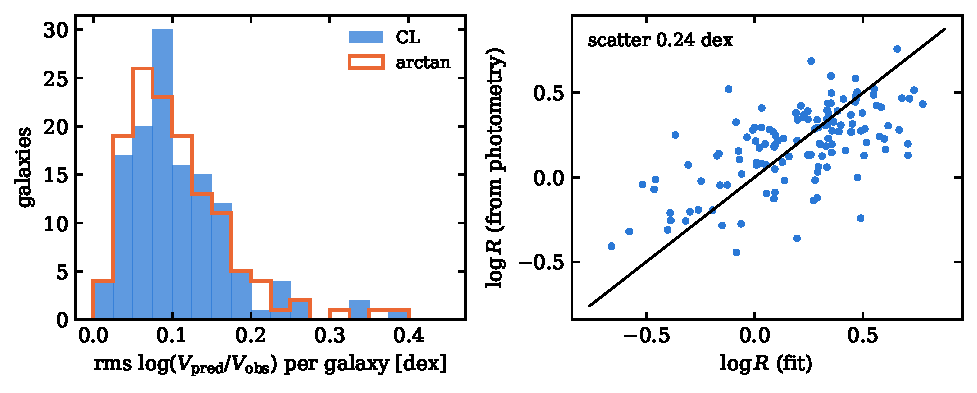
\includegraphics[width=0.84\textwidth]{fig/fig6_prediction.pdf}
\caption{Left: per-galaxy rms deviation of the rotation curves predicted from $(\Mbar,\Sin)$ for CL and arctan (leave-one-out calibration). Right: CL radius predicted from photometry against the fitted radius.}
\label{fig:pred}
\end{figure}

\section{Discussion}
\label{sec:disc}

\paragraph{What the CL parameters add.} The results separate cleanly into what belongs to the data and what belongs to the CL form. Both scaling relations, and the morphological trend of the inner scale, are present equally in a model-independent gradient and in the arctan control; they are properties of SPARC, as \citet{Lelli2013} and \citet{Lelli2016btfr} established. The CL form adds three things. Its inner gradient agrees in the median with the measured inner secant slope (median ratio $1.01$, against $1.38$ for arctan), and its plateau is a tight proxy of $\Vf$ ($\vL\simeq1.07\,\Vf$ with $0.03$\,dex scatter, against $0.05$\,dex for $V_c$). Its radius has a close model-independent counterpart in the one-third point of $v^2$ ($r_{1/3}\simeq0.9R$). And its inner branch is, up to the small Hubble term, a uniform sphere, so that Eq.~(\ref{eq:rho}) turns the central dynamical density of \citet{Lelli2013} into the mean density $3M/4\pi R^3$ of the CL core, while the BTFR concerns $M/R$. Both scaling relations then become statements about how two combinations of the same two parameters follow the light.

\paragraph{The fine-tuning question in CL terms.} \citet{Lelli2013} write the relation as $\log d_RV(0)=-0.2\mu_0+0.5\log[\beta G\,(M_{\rm bar}/L)/(\Delta z\,f_{\rm bar,0})]$, with $f_{\rm bar,0}$ the central baryon fraction and $\Delta z$ the thickness of the central component, and point out that a slope of exactly $-0.2$ implies that the bracket is constant from galaxy to galaxy. In the CL reading, $f_{\rm bar,0}=\rho_{\rm bar,0}/(3M/4\pi R^3)$, and a slope near $0.5$ per dex means that, if the thickness and mass-to-light ratio of the central component vary little, the central luminous density is close to a fixed fraction of the CL core density, with the remaining scatter of $\approx0.25$\,dex. Within the CL framework this is a definite question: why the core density $M/R^3$ of the fitted flow should follow the central stellar density. This paper documents the empirical fact; explaining it is left to the underlying theory.

\paragraph{Limitations.} (i) $\Sin$ is the surface brightness at the innermost tabulated radius, not a true extrapolation to $r=0$; its physical radius depends on resolution and distance. The extrapolated $\Sigma_{\rm ex}$ gives the same result. (ii) The photometry is 3.6\,$\mu$m rather than R band, so only slopes, not normalisations, can be compared with Eq.~(\ref{eq:lelli}); band-dependent mass-to-light variations may contribute to slope differences. (iii) $\sdat$ uses the first three points and is subject to beam smearing, as the SPARC curves are; distance errors scatter all gradients ($s\propto D^{-1}$) but not $\Sigma$. (iv) Only single-Lagrangian fits are used; 25 galaxies with unconstrained CL radius are excluded, and multi-region CL fits \citep{deHaas2026} are not considered. (v) $H_z$ is fixed; its effect on $\sCL$ is below 1\% here. (vi) The SPARC sample overlaps with that of \citet{Lelli2013}, so this is a confirmation of the relation in a model parametrisation, not an independent rediscovery. (vii) The paper does not use the embedding condition $GM/R^2=cH_z$ proposed by \citet{deHaas2025c}; in these fits the median $GM/R^2$ is $10^{-1.0}cH_z$, a point that a theoretical treatment of the BTFR within the CL framework will need to address.

\section{Conclusions}

The approach connects a relativistic, rapidity-based construction to galactic observations through a slow-flow reduction. The resulting CL rotation law is fitted to the kinematic data alone, and its parameters are then compared with baryonic properties not used in the fits. The present study therefore provides baryonic consistency tests of a theoretically motivated rotation-curve model. It does not derive the observed scaling relations from the underlying theory: why $M/R^3$ follows the central light, why $M/R$ follows $\Mbar$ with the observed slope, and why the characteristic acceleration lies about a factor of ten below $cH_z$ remain open. Within that scope:

\begin{enumerate}
\item The inner branch of the CL rotation curve is that of a homogeneous sphere up to the small Hubble term: $\sCL^2\simeq GM/R^3$ (exact for $H_z=0$), and $\rho_{\rm dyn,0}=3\sCL^2/4\pi G\simeq3M/4\pi R^3$ is the mean density of the CL core. $R$ is observable as the radius where $v^2$ reaches one third of its plateau.
\item Fitted to SPARC, the CL gradient reproduces the central velocity gradient--surface brightness relation of \citet{Lelli2013}: $\rho=0.76$, bisector slope $0.45$ ($0.41$--$0.50$) per dex at 3.6\,$\mu$m, with ordinary and inverse slopes of $0.35$ and $0.56$, provided the surface brightness includes the observed central light.
\item The CL plateau speed reproduces the BTFR with a scatter of $0.249$\,dex, close to the $0.226$\,dex obtained with $\Vf$, and $\vL$ tracks $\Vf$ to $0.03$\,dex.
\item A control with the arctan curve shows that both relations are properties of the data. The CL form is distinguished by an inner gradient that matches the measured secant slope in the median, a tight plateau proxy for $\Vf$ and the uniform-core identity, not by a stronger correlation or a better photometric prediction.
\item For the selected sample, the two SPARC relations jointly predict rotation curves from baryonic quantities to within a typical factor of $1.25$ ($0.097$\,dex) with either model, about three times the residual of a direct fit.
\end{enumerate}

\section*{Data and code availability}
SPARC data are from \citet{Lelli2016sparc}. All CL fits of the 175 SPARC galaxies, the scripts that produce every number, table and figure in this paper, and the per-galaxy results (\texttt{galaxies.csv}) are archived on Zenodo, doi:\codeDOI, with a working copy at \url{https://github.com/haas2u-ai/bq-galaxy-models}, folder \texttt{SPARC-CL-scaling}. Note that the present paper refits all 175 galaxies with its own code (a single CL curve fitted in $v^2$), so its per-galaxy results are those in \texttt{galaxies.csv}, not the earlier atlas fits. Appendix~\ref{app:repro} lists the steps.

\appendix
\section{Reproducibility}
\label{app:repro}
With Python~3 and NumPy, SciPy, pandas and Matplotlib installed, run from the folder \texttt{code/}:
\begin{enumerate}
\item \texttt{python cl\_lelli\_analysis.py} --- fits the CL and arctan models to all 175 galaxies, derives the gradients and surface-brightness proxies, and writes \texttt{data/galaxies.csv} and \texttt{data/results.json} (Tables~\ref{tab:lelli} and \ref{tab:btfr}, Sects.~\ref{sec:core}--\ref{sec:R}).
\item \texttt{python cl\_photometric\_prediction.py} --- leave-one-out photometric prediction, writes \texttt{data/prediction.json} (Sect.~\ref{sec:pred}).
\item \texttt{python cl\_vspace\_robustness.py} --- refits the CL model in velocity space and writes \texttt{data/robustness\_vspace.json} (Sect.~\ref{sec:fits}).
\item \texttt{python make\_figures.py} --- Figs.~\ref{fig:examples}--\ref{fig:pred}.
\end{enumerate}
The scripts read the original SPARC tables (\texttt{MassModels\_Lelli2016c.mrt} and \texttt{Table1wbulge.mrt}, the SPARC galaxy table with bulge luminosities appended) without modification.

\begin{thebibliography}{99}
\bibitem[Courteau(1997)]{Courteau1997} Courteau S., 1997, AJ, 114, 2402
\bibitem[de Haas(2018)]{deHaas2018} de Haas E.\,P.\,J., 2018, A `Constant Lagrangian' RMW-RSS quantified fit of the galaxy rotation curves of the complete SPARC database of 175 LTG galaxies, viXra:1908.0222
\bibitem[de Haas(2025a)]{deHaas2025a} de Haas E.\,P.\,J., 2025a, One single metric model's unifying perspective on four issues with galactic dynamics: B-TF relation, rotation curves, spirals and SMBH-growth, J. High Energy Phys. Grav. Cosmol., 11, 1252, doi:10.4236/jhepgc.2025.114078
\bibitem[de Haas(2025b)]{deHaas2025b} de Haas E.\,P.\,J., 2025b, The role of the Hubble parameter in galactic rotation curves and spiral morphology, J. High Energy Phys. Grav. Cosmol., 11, 1595, doi:10.4236/jhepgc.2025.114097
\bibitem[de Haas(2025c)]{deHaas2025c} de Haas E.\,P.\,J., 2025c, Galaxies as FRW-embedded systems: rapidity matching derivations of $a_0=cH$ and the BTFR, Zenodo, doi:10.5281/zenodo.17634641
\bibitem[de Haas(2026a)]{deHaas2026} de Haas E.\,P.\,J., 2026a, From rotation curves to cosmic time: probing high-redshift expansion through nested spiral dynamics, J. High Energy Phys. Grav. Cosmol., 12, 334, doi:10.4236/jhepgc.2026.121022
\bibitem[de Haas(2026b)]{deHaasGFD} de Haas E.\,P.\,J., 2026b, Three levels of a single vacuum-flow field equation: Newtonian gravity, the Hubble flow, and galactic rotation curves without dark matter, Zenodo, doi:10.5281/zenodo.20796685
\bibitem[de Haas(2026c)]{deHaasRapidity} de Haas E.\,P.\,J., 2026c, The gravitational rapidity potential: a Lorentz-rotor formulation of gravity from galactic dynamics to black-hole geodetic precession, Zenodo, doi:10.5281/zenodo.21082573
\bibitem[de Haas(2026d)]{deHaasMC} de Haas E.\,P.\,J., 2026d, The proper-time Maurer--Cartan connection in a rotor-generated Spin(1,3) theory of gravitation: a connection-level derivation of the constant-Lagrangian galactic rotation-curve law, Zenodo, doi:10.5281/zenodo.21242316
\bibitem[de Haas(2026e)]{deHaasSpin} de Haas E.\,P.\,J., 2026e, A Spin(1,3) rapidity theory for galactic rotation curves: kinematic and Maurer--Cartan derivations of the constant-Lagrangian condition, Zenodo, doi:10.5281/zenodo.21844437
\bibitem[Gullstrand(1922)]{Gullstrand1922} Gullstrand A., 1922, Allgemeine L\"osung des statischen Eink\"orperproblems in der Einsteinschen Gravitationstheorie, Ark. Mat. Astron. Fys., 16(8), 1
\bibitem[Hamilton \& Lisle(2008)]{Hamilton2008} Hamilton A.\,J.\,S., Lisle J.\,P., 2008, Am. J. Phys., 76, 519
\bibitem[Isobe et al.(1990)]{Isobe1990} Isobe T., Feigelson E.\,D., Akritas M.\,G., Babu G.\,J., 1990, ApJ, 364, 104
\bibitem[Lelli et al.(2013)]{Lelli2013} Lelli F., Fraternali F., Verheijen M., 2013, MNRAS, 433, L30
\bibitem[Lelli et al.(2016a)]{Lelli2016sparc} Lelli F., McGaugh S.\,S., Schombert J.\,M., 2016a, AJ, 152, 157
\bibitem[Lelli et al.(2016b)]{Lelli2016btfr} Lelli F., McGaugh S.\,S., Schombert J.\,M., 2016b, ApJ, 816, L14
\bibitem[Lelli et al.(2019)]{Lelli2019} Lelli F., McGaugh S.\,S., Schombert J.\,M., Desmond H., Katz H., 2019, MNRAS, 484, 3267
\bibitem[McGaugh et al.(2000)]{McGaugh2000} McGaugh S.\,S., Schombert J.\,M., Bothun G.\,D., de Blok W.\,J.\,G., 2000, ApJ, 533, L99
\bibitem[McGaugh et al.(2016)]{McGaugh2016} McGaugh S.\,S., Lelli F., Schombert J.\,M., 2016, Phys. Rev. Lett., 117, 201101
\bibitem[Painlev\'e(1921)]{Painleve1921} Painlev\'e P., 1921, La m\'ecanique classique et la th\'eorie de la relativit\'e, C. R. Acad. Sci. Paris, 173, 677
\bibitem[Wong \& Rivers(2016)]{Wong2016} Wong J.\,C.\,C., Rivers R.\,J., 2016, A baseline model for modified Newtonian mechanics I: the early Universe, arXiv:1601.00376
\end{thebibliography}

\end{document}
